\chapter{Server Configuration}
{
    \renewcommand*{\theenumi}{\thesubsection.\arabic{enumi}}
    \renewcommand*{\theenumii}{\theenumi.\arabic{enumii}}
    \renewcommand*{\theenumiii}{\theenumii.\arabic{enumiii}}

    \section{Description}
        The server will be responsible for hosting the web interface, as 
        well as holding the PostgreSQL database. The server will be attached 
        to the device.

    \section{Hardware}

        \subsection{Mainboard}
            Our server will be a Raspberry Pi, Model B. It was chosen due to the 
            small size, availability, price, and versatility. The Raspberry Pi 
            specs include:
            \begin{itemize}
                \item 700MHz ARM CPU
                \item 250MHz Broadcom VideoCore IV GPU
                \item 512 MB SDRAM
                \item 3.5” by 2”
                \item Various connection interfaces such as
                \begin{itemize}
                    \item Composite RCA
                    \item HDMI
                    \item 3.5 mm audio jack
                    \item 10/100 Ethernet LAN
                    \item GPIO
                    \item Two USB 2.0
                    \item SD Reader
                \end{itemize}
            \end{itemize}

            \begin{figure}[htb]
                \centering
                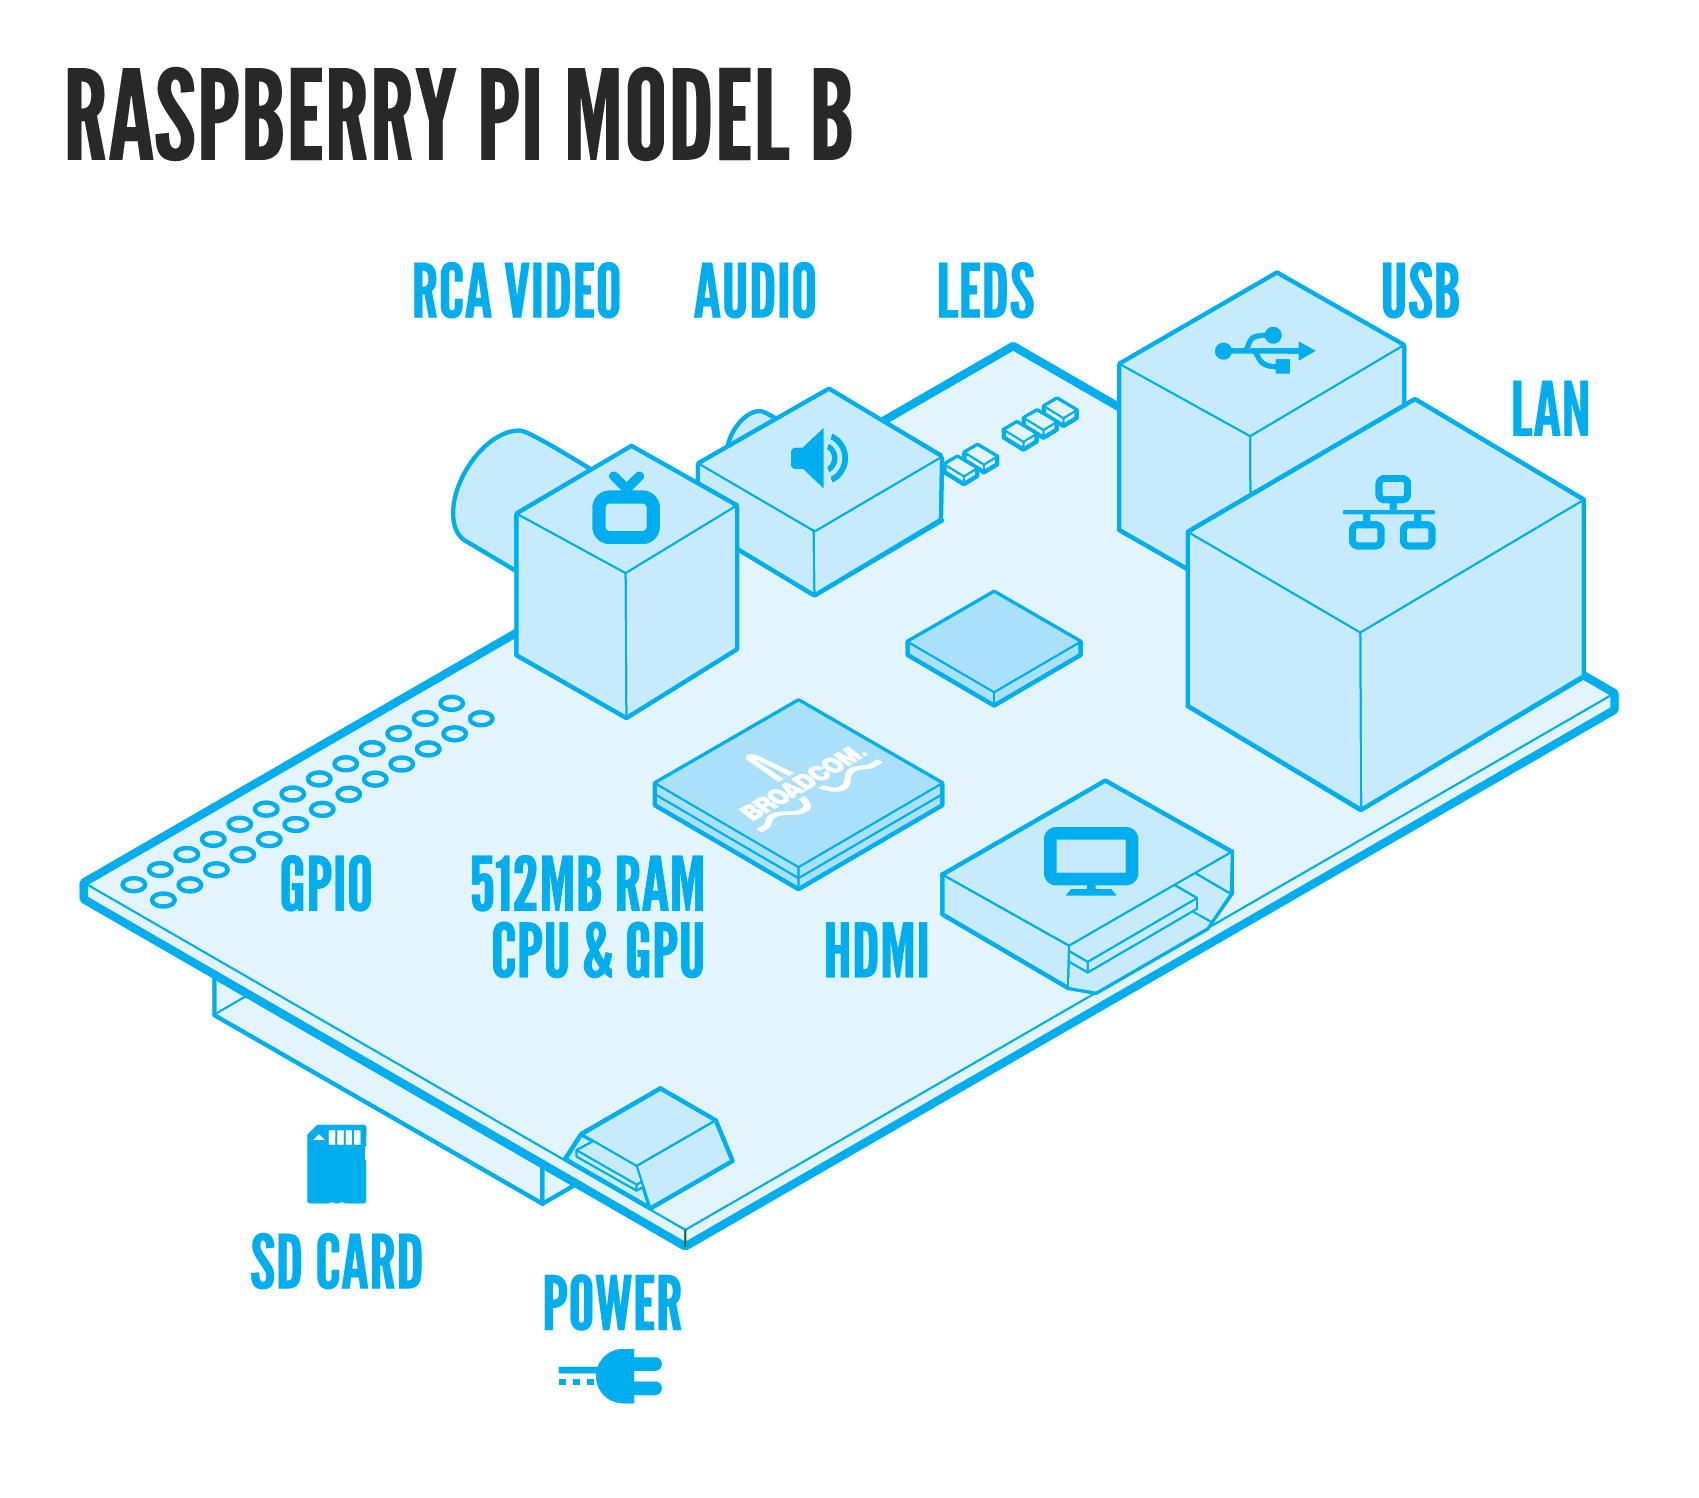
\includegraphics[width=0.9\textwidth]{Images/RaspberryPI.png}
                \caption{Diagram of Raspberry PI}
                \label{fig:RaspPi}
            \end{figure}


        \subsection{Storage}
            Onboard storage will be comprised of a 8GB Element 14 branded SD card. 
            This is the Raspberry Pi’s primary boot device, and will contain 
            the Operating System and all necessary software. Additional storage 
            can be obtained through USB storage devices if necessary. 

        \subsection{Power Supply}
            The Raspberry Pi will be powered via a 5 volt Element 14 branded 
            MicroUSB adapter. 

    \section{Software}
    
        \subsection{Raspian}
            Raspian is a Raspberry Pi optimized version of the Debian Linux 
            operating system. We have chosen Debian for its stability, and its 
            ability at handling the services we will be utilizing. Additional 
            packages will be handled using apt-get.

        \subsection{Apache2}
            We will use the Apache2 server software to handle the web interface. 
            We have chosen this due to its ease of use and stability. Apache2 
            will be integrating into PostgreSQL while handling web information.

        \subsection{PostgreSQL}
            We will be using PostgreSQL to handle database information, such as 
            user credentials and drink customizations. Any sensitive information 
            will be hashed and salted before being placed into the database. 
